% !TeX spellcheck = en_GB
% !TeX root = ../phd-thesis.tex

\begin{figure}
    \centering{
        \begin{subfigure}[t]{0.4\linewidth}
            \centering
            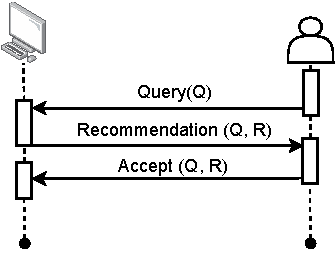
\includegraphics[width=\linewidth]{figures/quick-accept}
            \caption{Quick accept: the user accepts the recommendation without asking for explanations.}
            \label{fig:quick-accept}
        \end{subfigure}
        \hfill%\vline\hfill
        \begin{subfigure}[t]{0.4\linewidth}
            \centering
            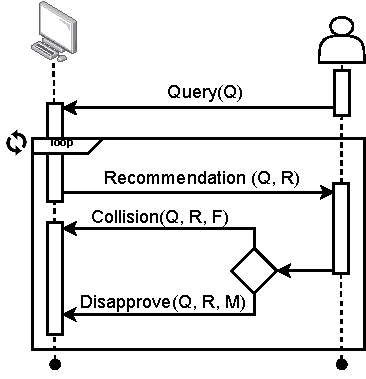
\includegraphics[width=\linewidth]{figures/quick-retry}
            \caption{Quick retry: the user rejects the recommendation without asking for explanations. Another recommendation is proposed, accordingly.}
            \label{fig:quick-retry}
        \end{subfigure}
    }

    \medskip

    \centering{
        \begin{subfigure}[t]{0.4\linewidth}
            \centering
            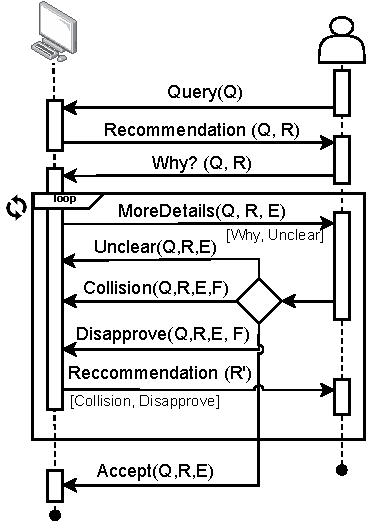
\includegraphics[width=\linewidth]{figures/explanation-loop}
            \caption{Ordinary explanation loop: the user asks `why' after a recommendation, and then agent answers with further details. The request for details may be repeated several times.}
            \label{fig:explanation-loop}
        \end{subfigure}
        \hfill%\vline\hfill
        \begin{subfigure}[t]{0.4\linewidth}
            \centering
            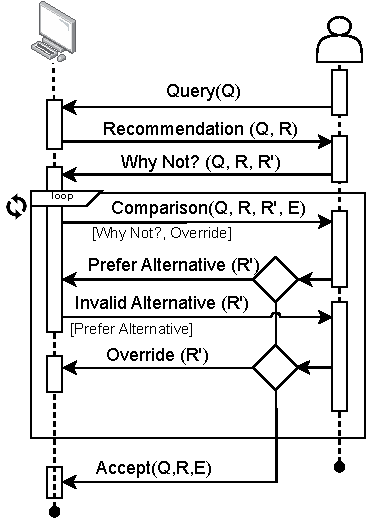
\includegraphics[width=\linewidth]{figures/contrastive-explanation-loop}
            \caption{Contrastive explanation loop: the user asks `why not' another recommendation. The agent may then explain why the other recommendation is acceptable or invalid. The user may either accept the original recommendation or prefer their own.}
            \label{fig:contrastive-explanation-loop}
        \end{subfigure}
    }
    \caption{Sequence diagrams describing most common scenarios of the protocol.}
    \label{fig:protocol-sequence-diagrams}
\end{figure}
